
\section{Applications and Domains}
\label{sec:applications}

Implicit and explicit feedback find applications across diverse domains, with feedback types influencing personalization strategies, user experience, and business outcomes. This section provides comprehensive analysis of how different feedback modalities shape recommendation systems in various industries and use cases.

\begin{figure}[ht]
\centering
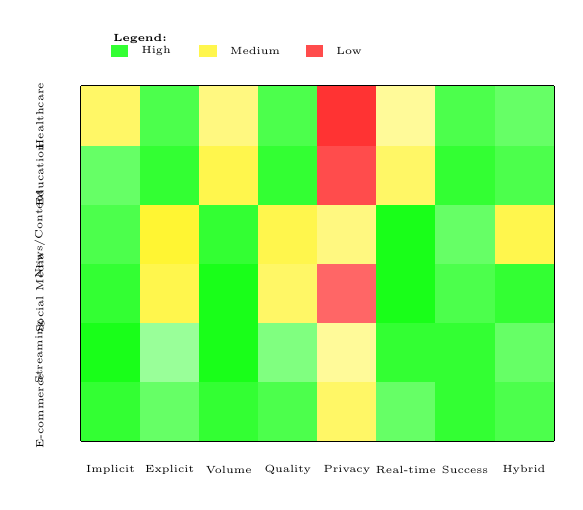
\begin{tikzpicture}[scale=0.75, transform shape]
    % Domain matrix
    \draw[thick] (0,0) grid (8,6);
    
    % Row headers - REDUCED SIZE
    \node[font=\tiny, rotate=90] at (-0.7,0.5) {E-commerce};
    \node[font=\tiny, rotate=90] at (-0.7,1.5) {Streaming};
    \node[font=\tiny, rotate=90] at (-0.7,2.5) {Social Media};
    \node[font=\tiny, rotate=90] at (-0.7,3.5) {News/Content};
    \node[font=\tiny, rotate=90] at (-0.7,4.5) {Education};
    \node[font=\tiny, rotate=90] at (-0.7,5.5) {Healthcare};
    
    % Column headers - REDUCED SIZE AND BETTER POSITIONING
    \node[font=\tiny] at (0.5,-0.5) {Implicit};
    \node[font=\tiny] at (1.5,-0.5) {Explicit};
    \node[font=\tiny] at (2.5,-0.5) {Volume};
    \node[font=\tiny] at (3.5,-0.5) {Quality};
    \node[font=\tiny] at (4.5,-0.5) {Privacy};
    \node[font=\tiny] at (5.5,-0.5) {Real-time};
    \node[font=\tiny] at (6.5,-0.5) {Success};
    \node[font=\tiny] at (7.5,-0.5) {Hybrid};
    
    % Content fills
    % E-commerce row
    \fill[green!80] (0,0) rectangle (1,1);
    \fill[green!60] (1,0) rectangle (2,1);
    \fill[green!80] (2,0) rectangle (3,1);
    \fill[green!70] (3,0) rectangle (4,1);
    \fill[yellow!60] (4,0) rectangle (5,1);
    \fill[green!60] (5,0) rectangle (6,1);
    \fill[green!80] (6,0) rectangle (7,1);
    \fill[green!70] (7,0) rectangle (8,1);
    
    % Streaming row
    \fill[green!90] (0,1) rectangle (1,2);
    \fill[green!40] (1,1) rectangle (2,2);
    \fill[green!90] (2,1) rectangle (3,2);
    \fill[green!50] (3,1) rectangle (4,2);
    \fill[yellow!40] (4,1) rectangle (5,2);
    \fill[green!80] (5,1) rectangle (6,2);
    \fill[green!80] (6,1) rectangle (7,2);
    \fill[green!60] (7,1) rectangle (8,2);
    
    % Social Media row
    \fill[green!80] (0,2) rectangle (1,3);
    \fill[yellow!70] (1,2) rectangle (2,3);
    \fill[green!90] (2,2) rectangle (3,3);
    \fill[yellow!60] (3,2) rectangle (4,3);
    \fill[red!60] (4,2) rectangle (5,3);
    \fill[green!90] (5,2) rectangle (6,3);
    \fill[green!70] (6,2) rectangle (7,3);
    \fill[green!80] (7,2) rectangle (8,3);
    
    % News row
    \fill[green!70] (0,3) rectangle (1,4);
    \fill[yellow!80] (1,3) rectangle (2,4);
    \fill[green!80] (2,3) rectangle (3,4);
    \fill[yellow!70] (3,3) rectangle (4,4);
    \fill[yellow!50] (4,3) rectangle (5,4);
    \fill[green!90] (5,3) rectangle (6,4);
    \fill[green!60] (6,3) rectangle (7,4);
    \fill[yellow!70] (7,3) rectangle (8,4);
    
    % Education row
    \fill[green!60] (0,4) rectangle (1,5);
    \fill[green!80] (1,4) rectangle (2,5);
    \fill[yellow!70] (2,4) rectangle (3,5);
    \fill[green!80] (3,4) rectangle (4,5);
    \fill[red!70] (4,4) rectangle (5,5);
    \fill[yellow!60] (5,4) rectangle (6,5);
    \fill[green!80] (6,4) rectangle (7,5);
    \fill[green!70] (7,4) rectangle (8,5);
    
    % Healthcare row
    \fill[yellow!60] (0,5) rectangle (1,6);
    \fill[green!70] (1,5) rectangle (2,6);
    \fill[yellow!50] (2,5) rectangle (3,6);
    \fill[green!70] (3,5) rectangle (4,6);
    \fill[red!80] (4,5) rectangle (5,6);
    \fill[yellow!40] (5,5) rectangle (6,6);
    \fill[green!70] (6,5) rectangle (7,6);
    \fill[green!60] (7,5) rectangle (8,6);
    
    % Legend - REPOSITIONED TO AVOID COLLISION
    \node[font=\tiny] at (1,6.8) {\textbf{Legend:}};
    \fill[green!80] (0.5,6.5) rectangle (0.8,6.7);
    \node[font=\tiny, anchor=west] at (0.9,6.6) {High};
    \fill[yellow!70] (2,6.5) rectangle (2.3,6.7);
    \node[font=\tiny, anchor=west] at (2.4,6.6) {Medium};
    \fill[red!70] (3.8,6.5) rectangle (4.1,6.7);
    \node[font=\tiny, anchor=west] at (4.2,6.6) {Low};
    
\end{tikzpicture}
\caption{Domain Application Matrix: Feedback Characteristics Across Industries}
\Description{A comprehensive matrix visualization comparing feedback characteristics across eight major application domains (E-commerce, Streaming, Social Networks, News, Education, Healthcare, Travel, Job Matching). The matrix displays scores for Implicit Availability (0-100\%), Explicit Quality (0-10), Privacy Concern (0-10), and overall Success Rating (0-10) for each domain, using a color-coded heatmap where darker colors represent higher values.}
\label{fig:domain_matrix}
\end{figure}

Figure~\ref{fig:domain_matrix} provides a comprehensive comparison of feedback characteristics across major application domains, illustrating how different industries leverage implicit and explicit feedback mechanisms with varying degrees of success and privacy considerations.

\subsection{E-commerce and Retail}

\subsubsection{Product Recommendation Systems}

E-commerce platforms leverage complex feedback ecosystems:

\begin{itemize}
    \item \textbf{Implicit Feedback Sources}: Clickstreams, browsing patterns, cart additions, purchase sequences, search queries, and time spent on product pages
    \item \textbf{Explicit Feedback Sources}: Product ratings, detailed reviews, wishlists, and return/refund feedback
    \item \textbf{Hybrid Integration}: Combining browsing intent with review validation for purchase prediction
\end{itemize}

Key challenges include:
\begin{itemize}
    \item \textbf{Abandonment Prediction}: Using implicit signals to identify at-risk shopping carts
    \item \textbf{Cross-Sell Optimization}: Recommending complementary products based on purchase patterns
    \item \textbf{Personalized Pricing}: Dynamic pricing based on user engagement and purchase history
    \item \textbf{Inventory Management}: Demand forecasting using implicit browsing trends
\end{itemize}

\subsubsection{Case Studies}

\textbf{Amazon's Recommendation Engine}:
\begin{itemize}
    \item Processes billions of implicit interactions daily
    \item "Customers who bought this also bought" uses collaborative filtering on purchase data
    \item "Frequently bought together" leverages co-purchase patterns
    \item Explicit reviews influence product ranking and visibility
    \item Hybrid models achieve 35\% of all purchases through recommendations
\end{itemize}

\textbf{Alibaba's Taobao Platform}:
\begin{itemize}
    \item Real-time implicit feedback processing for flash sales
    \item Social commerce integration with explicit friend recommendations
    \item Mobile-optimized implicit feedback (touch gestures, scroll patterns)
    \item Cross-border recommendation challenges with cultural feedback differences
\end{itemize}

\subsubsection{Performance Metrics}

E-commerce success metrics include:
\begin{itemize}
    \item \textbf{Conversion Rate}: Click-to-purchase ratios (typically 2-5\%)
    \item \textbf{Average Order Value}: Revenue impact of recommendations
    \item \textbf{Cart Completion Rate}: Reduction in abandonment through personalized suggestions
    \item \textbf{Return Rate}: Quality of recommendations measured by post-purchase satisfaction
\end{itemize}

\subsection{Content Streaming and Entertainment}

\subsubsection{Video Streaming Platforms}

Netflix, YouTube, and similar platforms rely heavily on implicit feedback:

\begin{itemize}
    \item \textbf{Implicit Signals}: Watch time, completion rates, skip behavior, pause patterns, rewind/fast-forward actions
    \item \textbf{Explicit Signals}: Thumbs up/down, ratings, reviews, playlist creation
    \item \textbf{Contextual Factors}: Time of day, device type, binge-watching patterns
\end{itemize}

Advanced applications include:
\begin{itemize}
    \item \textbf{Content Discovery}: Genre exploration based on viewing patterns
    \item \textbf{Binge Prediction}: Anticipating multi-episode consumption
    \item \textbf{Ad Insertion}: Optimal placement based on engagement patterns
    \item \textbf{Content Creation}: Using feedback to guide production decisions
\end{itemize}

\subsubsection{Music Streaming Services}

Spotify and Apple Music optimize for user engagement:

\begin{itemize}
    \item \textbf{Implicit Feedback}: Play counts, skip rates, playlist additions, repeat listens, share actions
    \item \textbf{Explicit Feedback}: Song ratings, playlist curation, artist follows, concert ticket purchases
    \item \textbf{Temporal Patterns}: Daily routines, mood-based listening, social sharing
\end{itemize}

Key innovations:
\begin{itemize}
    \item \textbf{Discover Weekly}: Algorithmic playlist generation from listening history
    \item \textbf{Blend Playlists}: Social music discovery through shared listening patterns
    \item \textbf{Mood Detection}: Inferring emotional state from music selection patterns
    \item \textbf{Live Performance Prediction}: Concert recommendations based on artist engagement
\end{itemize}

\subsubsection{Case Study: Netflix Recommendation System}

\begin{itemize}
    \item \textbf{Data Scale}: Processes 500+ billion user interactions daily
    \item \textbf{Implicit Dominance}: 95\% of viewing decisions based on implicit feedback
    \item \textbf{Personalized Thumbnails}: A/B testing different artwork based on user preferences
    \item \textbf{Row Personalization}: Dynamic content organization based on viewing history
    \item \textbf{Impact}: Accounts for 80\% of viewing time, prevents churn through engagement
\end{itemize}

\subsection{News and Content Platforms}

News recommendation represents a critical application domain with unique challenges arising from content velocity, diversity requirements, and editorial considerations. Unlike e-commerce or entertainment domains, news recommenders must balance personalization with information diversity, timeliness with quality, and engagement with societal responsibility.

\subsubsection{News Recommendation Characteristics}

News recommendation systems exhibit distinct properties that differentiate them from other domains:

\textbf{Temporal Dynamics and Content Freshness:} News articles have extremely short lifespans, with most content becoming obsolete within hours or days. Recommenders must prioritize recency while maintaining relevance, creating unique cold-start challenges for each new article~\cite{liu2010personalized}.

\textbf{Implicit Feedback Dominance:} News consumption generates rich implicit signals including click-through rates (CTR), dwell time, scroll depth, and sharing actions. Explicit feedback (ratings, likes) is rare in news contexts, making implicit signal processing crucial~\cite{okura2017embedding}. Dwell time proves particularly valuable, as longer reading sessions indicate genuine interest beyond clickbait engagement.

\textbf{Diversity and Filter Bubble Concerns:} News recommenders face heightened scrutiny regarding filter bubbles and echo chambers. Over-personalization risks limiting exposure to diverse viewpoints and important information outside user comfort zones~\cite{wu2019neural}. Balancing personalization with serendipity and diversity becomes a critical design objective with societal implications.

\subsubsection{Benchmark Datasets and Research Infrastructure}

The news recommendation community has developed several large-scale datasets that have become standard benchmarks:

\textbf{MIND Dataset (Microsoft News):} The MIND (Microsoft News Dataset)~\cite{wu2020mind_news} represents the largest publicly available news recommendation dataset, containing over 160,000 news articles and 15 million user interactions from Microsoft News. The dataset includes:
\begin{itemize}
    \item Rich article metadata: titles, abstracts, categories, entities, and contextual information
    \item User click histories spanning multiple weeks of behavior
    \item Comprehensive impression logs with both clicked and non-clicked articles
    \item Temporal information enabling time-aware recommendation evaluation
\end{itemize}

MIND has become the de facto standard for evaluating news recommendation algorithms, enabling reproducible research and fair algorithmic comparison. The dataset's scale and diversity support development of sophisticated deep learning models that leverage both content features and behavioral patterns.

\textbf{Adressa Dataset:} The Adressa dataset~\cite{gulla2017adressa} provides three months of user-article interactions from a Norwegian news portal, including:
\begin{itemize}
    \item Detailed reading session information with precise timestamps
    \item Fine-grained engagement metrics including scroll depth and active time
    \item User demographics and contextual information
    \item Article content, metadata, and editorial categorization
\end{itemize}

Adressa's strength lies in its detailed engagement metrics beyond simple clicks, enabling research on attention modeling and content quality assessment. The dataset supports investigation of reading patterns, session-based recommendation, and the relationship between engagement depth and genuine interest.

\subsubsection{Neural Approaches for News Recommendation}

Modern news recommendation has been transformed by neural architectures that effectively model both content semantics and user behavior:

\textbf{Content-Based Neural Modeling:} Neural news recommendation systems leverage pre-trained language models and attention mechanisms to understand article content~\cite{wu2019neural, wu2021empowering}. These approaches:
\begin{itemize}
    \item Extract semantic representations from titles, abstracts, and full text
    \item Identify salient entities, topics, and themes
    \item Model hierarchical article structure (words $\rightarrow$ sentences $\rightarrow$ documents)
    \item Leverage knowledge graphs for entity-aware recommendation
\end{itemize}

\textbf{Personalized Attention Mechanisms:} NPA (Neural News Recommendation with Personalized Attention)~\cite{wu2019npa} introduced user-specific attention networks that identify which aspects of news articles resonate with individual users. This approach recognizes that different users focus on different elements (e.g., some prioritize headlines, others prefer detailed analysis), enabling more nuanced personalization.

\textbf{Multi-View Learning:} Neural methods with attentive multi-view learning~\cite{wu2019neural} simultaneously process multiple article representations:
\begin{itemize}
    \item Textual content (titles, abstracts, bodies)
    \item Categorical information (topics, categories)
    \item Entity knowledge (named entities, knowledge graph embeddings)
    \item Temporal signals (publication time, trending status)
\end{itemize}

\textbf{Graph-Based Modeling:} Recent work applies graph neural networks to news recommendation~\cite{hu2020graph}, modeling:
\begin{itemize}
    \item User-article interaction graphs capturing historical preferences
    \item Article-article similarity graphs based on content and co-engagement
    \item User-user social graphs when available
    \item Temporal graphs capturing evolution of news topics and user interests
\end{itemize}

\subsubsection{Causal Inference and Debiasing}

News recommendation faces significant bias challenges that require causal inference approaches~\cite{qi2021causal}:

\textbf{Position Bias:} Articles shown in prominent positions receive disproportionate clicks regardless of relevance. Causal models help disentangle genuine interest from positional effects, enabling more accurate preference learning.

\textbf{Selection Bias:} Users self-select which articles to read, creating biased training data. Inverse propensity scoring and doubly robust estimation techniques address this challenge, improving offline evaluation reliability.

\textbf{Exposure Bias:} Limited article exposure means many relevant items never receive feedback. Causal inference helps estimate counterfactual preferences for unobserved articles, reducing popularity bias and improving long-tail recommendation.

\textbf{Clickbait and Engagement Quality:} Implicit feedback (clicks) can be misleading when sensationalist headlines drive clicks but disappoint readers. Dwell time, scroll depth, and return visit patterns provide more reliable quality signals, requiring multi-objective optimization balancing CTR with engagement depth.

\subsubsection{News Recommendation Challenges}

News platforms face several critical challenges beyond standard recommendation problems:

\begin{itemize}
    \item \textbf{Implicit Feedback}: Click-through rates, dwell time, scroll depth, sharing actions
    \item \textbf{Explicit Feedback}: Article ratings (rare), topic preferences, follow actions, report buttons
    \item \textbf{Quality Signals}: Time spent reading, return visits, bookmarking behavior, commenting activity
\end{itemize}

Critical considerations:
\begin{itemize}
    \item \textbf{Filter Bubble Mitigation}: Balancing personalization with diversity to prevent echo chambers
    \item \textbf{Fake News Detection}: Using engagement patterns and content analysis to identify misinformation
    \item \textbf{Editorial Control}: Maintaining editorial priorities alongside algorithmic recommendations
    \item \textbf{Breakthrough Discovery}: Introducing users to new topics and perspectives beyond their established interests
    \item \textbf{Real-time Adaptation}: Responding to breaking news and rapidly evolving trending topics
    \item \textbf{Serendipity}: Surprising users with unexpected but valuable content
\end{itemize}

\subsubsection{Industry Applications and Case Studies}

Major news platforms have developed sophisticated recommendation systems:

\textbf{Microsoft News:} Leverages the MIND dataset infrastructure in production, employing transformer-based models with personalized attention for billions of daily recommendations across global markets.

\textbf{Google News:} Combines collaborative filtering with content-based methods, using BERT-based models for semantic understanding and user interest modeling at scale.

\textbf{Apple News:} Focuses on editorial curation enhanced by algorithmic personalization, balancing human judgment with implicit feedback signals to maintain content quality.

\textbf{Yahoo News:} Pioneered early work in news recommendation, with continued focus on user engagement prediction and contextual bandits for real-time optimization.

\subsubsection{Social News Platforms}

Reddit and similar platforms use community feedback for news curation:

\begin{itemize}
    \item \textbf{Implicit Signals}: Upvote timing, comment engagement, subreddit subscriptions, crosspost patterns
    \item \textbf{Explicit Signals}: Direct voting feedback, moderator actions, community guidelines enforcement
    \item \textbf{Social Dynamics}: Influence propagation through social networks, viral content identification
    \item \textbf{Community Intelligence}: Leveraging collective wisdom for content quality assessment
\end{itemize}

\subsubsection{Future Directions in News Recommendation}

Emerging research directions include:

\begin{itemize}
    \item \textbf{Multimodal Integration:} Incorporating images, videos, and audio in news understanding
    \item \textbf{Cross-lingual Recommendation:} Enabling news discovery across language barriers
    \item \textbf{Fact-Checking Integration:} Automated verification as a recommendation signal
    \item \textbf{Longitudinal Interest Modeling:} Understanding how news interests evolve over time
    \item \textbf{Contextual Adaptation:} Location, time-of-day, and device-aware recommendations
    \item \textbf{Explainable News Recommendation:} Transparent reasoning for editorial trust
\end{itemize}

\subsection{Social Media and Networking}

\subsubsection{Content Ranking Algorithms}

Facebook, Twitter, and Instagram optimize for engagement:

\begin{itemize}
    \item \textbf{Implicit Feedback}: Likes, shares, comments, view duration, profile visits
    \item \textbf{Explicit Feedback}: Follow/unfollow actions, content reports, privacy settings
    \item \textbf{Network Effects}: Social graph analysis and influence propagation
\end{itemize}

Key applications:
\begin{itemize}
    \item \textbf{Feed Personalization}: Algorithmic content ranking for individual users
    \item \textbf{Ad Targeting}: Precise audience segmentation based on behavioral patterns
    \item \textbf{Community Detection}: Identifying interest groups and social clusters
    \item \textbf{Influence Maximization}: Optimizing content spread through social networks
\end{itemize}

\subsubsection{Case Study: Twitter's Algorithm}

\begin{itemize}
    \item \textbf{Multi-Objective Optimization}: Balancing engagement, relevance, and recency
    \item \textbf{Implicit Signals}: Retweet patterns, quote tweet behavior, thread engagement
    \item \textbf{Real-time Processing}: Adapting to trending topics and breaking news
    \item \textbf{Conversation Health}: Promoting constructive dialogue through feedback analysis
\end{itemize}

\subsection{Emerging Domains and Applications}

\subsubsection{Educational Platforms}

Learning management systems use feedback for personalization:

\begin{itemize}
    \item \textbf{Implicit Feedback}: Time spent on materials, quiz attempt patterns, navigation sequences
    \item \textbf{Explicit Feedback}: Course ratings, assignment feedback, learning goal declarations
    \item \textbf{Adaptive Learning}: Personalizing content difficulty and pacing based on engagement
\end{itemize}

\subsubsection{Health and Fitness Applications}

Wellness apps optimize for behavior change:

\begin{itemize}
    \item \textbf{Implicit Feedback}: Workout completion, step counts, sleep patterns, app usage frequency
    \item \textbf{Explicit Feedback}: Goal setting, satisfaction surveys, pain level reporting
    \item \textbf{Motivation Systems}: Using engagement patterns to provide timely encouragement
\end{itemize}

\subsubsection{Professional Networking}

LinkedIn and similar platforms focus on career development:

\begin{itemize}
    \item \textbf{Implicit Feedback}: Profile view patterns, connection requests, content engagement
    \item \textbf{Explicit Feedback}: Endorsements, recommendations, skill assessments
    \item \textbf{Career Path Prediction}: Using interaction patterns to suggest professional development
\end{itemize}

\subsubsection{Gaming and Interactive Entertainment}

Game platforms personalize player experiences:

\begin{itemize}
    \item \textbf{Implicit Feedback}: Play time, level completion, in-game purchases, social interactions
    \item \textbf{Explicit Feedback}: Game ratings, review comments, friend recommendations
    \item \textbf{Dynamic Difficulty}: Adjusting challenge levels based on player skill patterns
\end{itemize}

\subsection{Domain-Specific Feedback Characteristics}

\subsubsection{Feedback Abundance and Quality}

Different domains exhibit varying feedback landscapes:

\begin{table}[h]
\centering
\caption{Feedback Characteristics Across Domains}
\label{tab:domain_feedback}
\begin{tabular}{@{}lcccc@{}}
\toprule
Domain & Implicit Volume & Explicit Quality & Real-time Needs & Privacy Sensitivity \\
\midrule
E-commerce & Very High & High & Medium & Medium \\
Video Streaming & Extremely High & Medium & High & Low \\
Music Streaming & High & Medium & High & Low \\
News & High & Low & Very High & Medium \\
Social Media & Very High & Low & Very High & High \\
Education & Medium & High & Low & High \\
Health/Fitness & High & Medium & Medium & Very High \\
Professional & Medium & High & Low & High \\
Gaming & High & Medium & High & Medium \\
\bottomrule
\end{tabular}
\end{table}

\subsubsection{Cross-Domain Feedback Transfer}

Understanding feedback patterns across domains enables transfer learning:

\begin{itemize}
    \item \textbf{Music to Video}: Audio preferences predicting visual content interests
    \item \textbf{Shopping to Entertainment}: Purchase patterns informing content recommendations
    \item \textbf{Social to Professional}: Network behavior patterns in career contexts
    \item \textbf{Educational to Gaming}: Learning patterns informing game personalization
\end{itemize}

\subsection{Industry Best Practices and Implementation}

\subsubsection{Data Pipeline Architecture}

Successful implementations require robust infrastructure:

\begin{itemize}
    \item \textbf{Real-time Processing}: Streaming analytics for immediate feedback incorporation
    \item \textbf{Scalable Storage}: Distributed databases handling massive feedback volumes
    \item \textbf{Privacy Compliance}: GDPR/CCPA-compliant data handling and user consent management
    \item \textbf{A/B Testing Frameworks}: Continuous experimentation and performance monitoring
\end{itemize}

\subsubsection{Model Deployment and Monitoring}

Production systems require careful management:

\begin{itemize}
    \item \textbf{Online Learning}: Continuous model updates with new feedback
    \item \textbf{Performance Monitoring}: Real-time tracking of recommendation quality metrics
    \item \textbf{Fallback Strategies}: Graceful degradation when feedback signals are weak
    \item \textbf{Bias Detection}: Ongoing monitoring for unfair or discriminatory patterns
\end{itemize}

\subsubsection{User Experience Optimization}

Feedback integration affects user satisfaction:

\begin{itemize}
    \item \textbf{Seamless Integration}: Implicit feedback collection without disrupting user flow
    \item \textbf{Transparency}: Clear communication about how feedback influences recommendations
    \item \textbf{Control Mechanisms}: User options to adjust feedback sensitivity and preferences
    \item \textbf{Privacy Controls}: Granular permissions for different feedback types
\end{itemize}

\subsection{Impact on Business Outcomes}

\subsubsection{Quantitative Benefits}

Successful feedback integration drives measurable improvements:

\begin{itemize}
    \item \textbf{Revenue Impact}: 15-35\% increase in conversion rates through personalized recommendations
    \item \textbf{User Engagement}: 20-50\% improvement in session duration and return visits
    \item \textbf{Customer Satisfaction}: Higher NPS scores through relevant personalization
    \item \textbf{Operational Efficiency}: Reduced support costs through proactive recommendations
\end{itemize}

\subsubsection{Qualitative Benefits}

Beyond metrics, feedback systems provide strategic advantages:

\begin{itemize}
    \item \textbf{Competitive Differentiation}: Superior personalization as a market advantage
    \item \textbf{Customer Loyalty}: Building long-term relationships through understanding
    \item \textbf{Innovation Opportunities}: Data-driven insights for product development
    \item \textbf{Risk Mitigation}: Early detection of user dissatisfaction and churn signals
\end{itemize}

\subsection{Future Domain Evolution}

Emerging trends will reshape feedback utilization:

\begin{itemize}
    \item \textbf{Metaverse Integration}: Spatial and embodied feedback in virtual environments
    \item \textbf{IoT Ecosystem}: Connected device feedback for holistic user understanding
    \item \textbf{Brain-Computer Interfaces}: Direct neural feedback for ultimate personalization
    \item \textbf{Quantum Computing}: Massive-scale feedback processing for unprecedented accuracy
\end{itemize}

This comprehensive analysis demonstrates how feedback types fundamentally shape recommendation system design and outcomes across diverse application domains, with each domain requiring tailored approaches to maximize effectiveness and user satisfaction.
